
\appendix

%%%%%%%%%%%%%%%%%%%%%%%%%%%%%%%%%%%%%%%%%%%%%%%%
% Apendice A
%%%%%%%%%%%%%%%%%%%%%%%%%%%%%%%%%%%%%%%%%%%%%%%%
\chapter{Edad escolar en diferentes Sistemas Educativos}\label{anexo:edad-educacion}

Incluso en la Unión Europea, los Sistemas Educativos difieren en la edad de escolarización de los estudiantes. Por ello, se ha confeccionado una tabla que intenta resumir la edad estándar en la que un niño está escolarizado durante las distintas etapas educativas\footnote{Se hablará de las etapas en las que el Sistema Educativo referido está bajo la responsabilidad del Ministerio de Educación (o equivalente) del propio país. Esto no excluye a la educación en centros privados.}. La información está basado en \cite{cursos-educacion-europa}.

Se tomará como referencia las etapas del Sistema Educativo Español para mostrar los años que pasan los estudiantes. Con respecto a la selección de países para realizar la comparación, se escogen los más representativos en los que se han realizado los estudios sobre el aprendizaje de la programación y donde más extendido están las plataformas que se mencionan en el presente documento. 


\begin{table}[!ht]
	\begin{centering}
		\begin{tabular}{c|c|c|c|c}
\emph{País} & Infantil & Primaria & Secundaria & Bachillerato\\
\hline
\emph{España} & 0-6 & 6-12 & 12-16 & 16-18\\
\emph{Estados Unidos} & 3-6 & 6-10 & 10-14 & 14-18\\
\emph{Reino Unido} & 2-5 & 5-11 & 11-16 & 16-18\\
\emph{Alemania} & 0-6 & 6-10 & 10-16 & 16-19\\
\emph{Francia} & 2-6 & 6-11 & 11-16 & 16-18\\
\emph{Bélgica} & 0-2.5/3 & 2.5/3-6 & 6-12 & 12-18\\
\emph{Irlanda} & 4-6 & 6-12 & 12-15 & 15-19\\
\end{tabular}
	\caption{Comparativa de edades de escolarización en diferentes Sistemas Educativos con respecto a las etapas del Sistema Educativo Español.}
		\label{tab:comparativa-tecnicas}
	\end{centering}
\end{table}

En el caso del Sistema Educativo Americano, existen muchas vías en la formación de un niño, como bien detalla A. Corsi-Bunker en\cite{guide-education-us}. Dependiendo de si se escoge una vía privada o dependiendo del estado, los años pueden variar. Aún así, en la tabla \ref{tab:comparativa-tecnicas} se muestra el modelo estándar (sistema K-12). En la figura \ref{fig:education-usa} se puede ver más en detalle esta diferencia.

\begin{figure}[!ht]
	\begin{centering}
		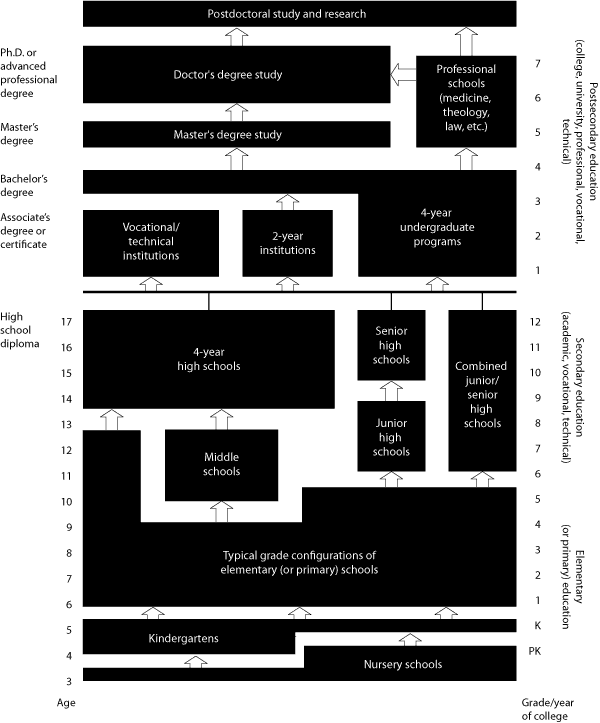
\includegraphics[width=0.8\textwidth]{images/education-usa.png}
			\caption{Tabla que muestra los típicos patrones de progresión en el Sistema Educativo Americano. Fuente: U.S. Department of Education, National Center for Education Statistics, Annual Reports Program. Obtenido de \url{http://nces.ed.gov/programs/digest/d11/figures/fig_01.asp}}
				\label{fig:education-usa}
	\end{centering}
\end{figure}





%%%%%%%%%%%%%%%%%%%%%%%%%%%%%%%%%%%%%%%%%%%%%%%%
% Apendice B
%%%%%%%%%%%%%%%%%%%%%%%%%%%%%%%%%%%%%%%%%%%%%%%%
\chapter{Lenguaje Logo. Un resumen}\label{anexo:lenguaje-logo}

En esta sección se realizará un pequeño resumen de las características el lenguaje Logo para tener una visión general de su funcionamiento y sintaxis. Este resumen se ha basado en el trabajo de \cite[p.274-305]{feurzeig1969programming}. Si el lector quiere ampliar información sobre el lenguaje Logo, puede consultar \cite{friendly2014advanced} o en \cite{logo-resources}.


\subsection*{\texttt{Words}, \texttt{Sentences} y operaciones}

Un tipo de dato \emph{words} está formado por 0 o más caracteres sin espacios. Algunos ejemplos son: "SUN", "CAT", "97&!", "" (cadena vacía). En cambio, el tipo de datos \emph{sentences} es formado por un conjunto de \emph{words} separado por espacios, como por ejemplo "HELLO WORLD" o "3 + 2 = 5". 

En el lenguaje Logo existen operadores para tratar con los tipos \emph{words} y \emph{sentences}. Estos son \texttt{FIRST}, \texttt{LAST}, \texttt{BUTFIRST}, \texttt{BUTLAST}, \texttt{WORD} y \texttt{SENTENCE}. Estos operadores reciben una entrada y devuelven una salida. En la tabla \ref{tab:logo-operadores} se pueden ver ejemplos ilustrativos de su funcionamiento.

\begin{table}[!ht]
	\begin{centering}
		\begin{tabular}{c|c|c}
\emph{Operador} & Entrada & Salida\\
\hline
\texttt{FIRST} & "CAT" & "C"\\
\texttt{FIRST} & "CAT AND DOG" & "CAT"\\
\texttt{LAST} & "CAT" & "T"\\
\texttt{LAST} & "CAT AND DOG" & "DOG"\\
\texttt{BUTFIRST} & "CAT" & "AT"\\
\texttt{BUTFIRST} & "CAT AND DOG" & "AND DOG"\\
\texttt{BUTLAST} & "CAT" & "CA"\\
\texttt{BUTLAST} & "CAT AND DOG" & "CAT AND"\\
\texttt{WORD} & "CAT" "DOG" & "CATDOG"\\
\texttt{WORD} & "CAT " "DOG" & \emph{(Mensaje de error)}\\
\texttt{SENTENCE} & "CAT" "DOG" & "CAT DOG"\\
\texttt{SENTENCE} & "CAT " "DOG" & "CAT DOG"\\
\end{tabular}
	\caption{Tabla que muestra el funcionamiento de los operadores en el lenguaje Logo a través de ejemplos.}
		\label{tab:logo-operadores}
	\end{centering}
\end{table}





\subsection*{Operaciones}


\subsection*{Comandos}


\subsection*{Nombres}






























